% !TEX root = thesis.tex
\chapter{関連研究}
\section{Web工学と機械学習}
この節では、Web工学における課題をいくつか例示し、それらの課題を解決するために、機械学習がどのように用いられてきたかを概観する。
\subsection{Recommendation System}
主にWebショッピングを含むサイトや、Web広告の配信において求められる技術である。Webサイトを閲覧しているユーザに対し、そのユーザが購入したいと商品を予測して、Web上の広告などの形で推薦する。適切な広告を表示することにより、ユーザの購買行動を促進することが出来る。
Recommendation Systemの研究は、1992年のTapestryシステムに始まる\cite{goldberg1992using}。また、少なくとも90年代の終わりには、Amazon.com, CDNOW, eBay, Levis, GroupLensなど、様々なサイトにてRecommendation Systemは利用されていた\cite{resnick1997recommender}。
Recommendation Systemを実現するための、機械学習のテクニックとしては、大きく2種類が挙げられる\cite{koren2009matrix}。1つは、Content Filteringと呼ばれ、ユーザや商品の属性や購買傾向を学習することことで、推薦を行う。もう1つはCollaboraitive Filteringと呼ばれており、ユーザや商品の属性を扱う代わりに、購入や評価といった、ユーザの過去の行動を基にして、推薦を行う。
\subsection{Link Prediction}
Link Predictionとは、グラフが与えられたとき、現在のグラフ構造(ノード間接続の様子)から、未来の構造を予測する問題である。最初に提唱された論文\cite{liben2007link}では、ソーシャルネットワークの状態が与えられたとき、ユーザ間で交わされる将来の行動を予測する問題として述べられている。この論文では、ノード(ユーザ)間の近さを定義する方法や、全てのエッジ(接続)を通しで見て判断する方法、クラスタリングによる方法などが用いられている。論文で用いられているノード間の近さの定義を挙げる(\cite{liben2007link}より引用)。ノード$x$に対し、$x$とつながっているノードの集合を$Γ(x)$とする。\par
\begin{eqnarray}
graph distance & 
\end{eqnarray}
LInk Predictionには様々な応用が考えられる。ショッピングサイトのデータ分析に役立ったり\cite{clauset2004finding}、。Web工学の問題以外にも応用が可能であり、タンパク質の反応予測(Protein to Protein Interaction, PPI)に用いられたり\cite{bader2003gaining}、テロリストのネットワークや草原の食物連鎖の分析にも役に立っている\cite{clauset2008hierarchical}。
[加筆]
\subsection{Sentiment Analysis}
ユーザの感想データを手に入れられるようになってきた\\
事実だけでなく、他の人がどのような感情を抱いているのかを分析したい\\
opinion miningという語も広義には似た内容を指している\\
2001-2003に研究が出始めた\\
common neighbors\\
Jaccard係数 SVDによる次元削減\\
Stanfordによるデモに言及

\subsection{Learning to Rank}
多様なランキング素因を組み合わせて、ランキング関数を作成\\
→どの組み合わせが有効か、機械学習する

\section{機械学習で利用される、代表的な分類器}
機械学習のプロセスは、「入力データを、数学的モデルで使える素性に変換する」「素性を数学的モデルに入力して、出力値を得る」「出力を見ながら、モデルを修正する」という行程に大きく分けられる。データの分類問題を機械学習で解く場合、モデルによる出力値が分類結果に対応するよう、モデルを学習させることになる。この場合、モデルのことを分類器とも呼ぶ。\par
機械学習において、素性への変換部分は、データの種類に大きく依存する。一方、分類器に用いる数学的モデルと、モデルの改修法、つまり学習法は、汎用的に使うことができる。あるいは、画像や音声、文章といったデータの多様性を、素性という一般的な数値に落とし込むことで吸収して、汎用的分類モデルでも学習できるようにしている。\par
Deep Learning、あるいはDeep Neural Network(多層ニューラルネットワーク)は、汎用的分類モデルの一種である。ここでは、Deep Learningの他にどのような分類器が存在するのか、代表的なものを述べる。
%\subsection{線形識別モデル}

%\subsection{ロジスティック回帰}

\subsection{Support Vector Machine}
Support Vector Macine(SVM)は、図\ref{c2_svm}のように、データを2つのクラスに分類する能力を持ったモデルである\cite{cortes1995support-vector}。\par
SVMのメインとなる原理は、マージン最大化である。図\ref{c2_svm}は最も単純なSVMの問題を表しており、グラフ上に散らばった黒と白の点を、直線を1本引くことで分けることが目標である。言い換えれば、どの点が黒で、どの点が白なのかを識別する、2クラス分類問題を解こうとしている。緑の線は、分類に失敗している。青の線は分類に成功しているが、後から点線で表された新しい白点が加わると、やはり分類に失敗してしまう。赤の線は、現在見えている点を分類できるだけでなく、新しい点が加わっても正しく識別できる可能性が高い。SVMのマージン最大化とは、各点からの距離(マージン)の和が、最大になるように直線の引き方を決めることである。こうすることにより、汎化性能(訓練時に見えていなかった、新しいデータを正しく分類する性能)が最大になることが知られている。\par
この図のSVMは、データが直線で完全に分類できることを前提にしている。しかし、現実のデータは、\ref{c2_svm_mixed}のように、必ずしも1本の直線にて分類が可能ではない。(3次元以上の場合で言えば、1つの超平面にて分類が可能とは限らない。)このような場合に対応するため、まず非線形関数にてデータを高次元の空間に移し、超平面による分類が出来るように変換する方法が知られている\cite{burges1998tutorial}。ただし、一般に複雑な分類ほど、変換先の次元数が高くなる傾向があり、次元数が増えると、「次元の呪い」と言って、内積計算にかかる時間が指数関数的に増大することがわかっている\cite{bellman1961adaptive}。この計算時間を減少させるため、数式処理によって内積を計算する必要がなくなるように設計された、カーネル関数と呼ばれる変換関数を用いる方法が使われている(カーネルマジック)。
\begin{figure}[tbp]
 \centering
  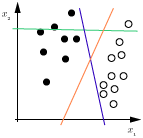
\includegraphics[width=80mm]{img/c2/svm}
 \caption{Support Vector Machineのマージン最大化}
 \label{c2_svm}
\end{figure}
\begin{figure}[tbp]
 \centering
  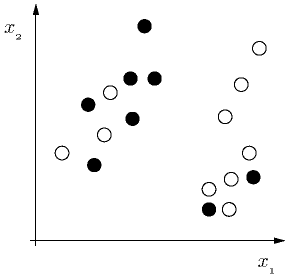
\includegraphics[width=80mm]{img/c2/svm_mixed}
 \caption{直線にて分類できない場合}
 \label{c2_svm_mixed}
\end{figure}
SVMは、広くその信頼性が認められたモデルの1つであり、ライブラリの利用方法も確立している。例えば、libsvm\footnote{\url{http://www.csie.ntu.edu.tw/~cjlin/libsvm/}}やliblinear\footnote{\url{http://www.csie.ntu.edu.tw/~cjlin/liblinear/}}は使用が容易なライブラリとしてよく知られている。これらのライブラリを使うと、簡単な所定の方式に沿って入力データファイルを用意し、CUI上で2,3回の操作をするだけで、SVMによる分類を行わせることができる。このとき、利用者が自分でプログラムを書く必要は全くない。プログラムを書かないで済むと、手軽に利用することができ、またバグを起こす危険性が非常に少なく安全に使うことができる。\par
Deep Learningについては、このようなライブラリはまだ存在していないため、Deep Learningの代表的なアルゴリズムについて、プログラム無しで利用できるようなライブラリの整備が望まれる。
\subsection{ニューラルネットワーク}
ニューラルネットワークは、人間の脳の構造を模倣した数学的モデルである。人間の脳は、ニューロンと呼ばれる神経細胞が大量に接続されて出来ている。ニューロンが電気信号を伝達することで、様々な脳の働きが行われている、と考えられている。プログラム上で表現されるニューラルネットワークには、人間の脳の動作との相違点もあり、脳が行っている計算を正しくシミュレートしているとは言い難い面もある\cite{kawato1998}が、機械学習のモデルとしては広く使われてきた。\par
\subsubsection{ニューラルネットワークの伝達方式}
以後、機械学習におけるニューラルネットワークのニューロンを、慣例に従ってユニットと呼ぶことにする。ニューラルネットワークでは、ユニットからユニットへの接続が網目のように広がっている。ユニットは入出力の機能を持つ。これは、生体におけるニューロンが、他のニューロンから化学的な刺激を受け取り、受け取った刺激に応じて自らも他のニューロンを刺激する構造を真似ている。ユニットは入力を受け取ると、活性化関数(activation function)を使って入力値を変換し、接続先のユニットへ出力する。このとき、ユニットからユニットへの結線に、重み(weight)と呼ばれる係数を付与して、出力を変化させることが普通である。これは、生体のニューロン同士の接続が、脳の学習につれて強固になり、刺激がより伝わりやすくなっていくことに対応させている。
\subsubsection{パーセプトロン}
パーセプトロンとは、ニューラルネットワークの一種である。複数のユニットをまとめた層(レイヤー)が、いくつか重なって出来ており、値の伝達は入力レイヤーから出力レイヤーへの一方向に限られているものを指す(feed-forward)。狭義には、単層かつ活性化関数にヘビサイド関数を用いた2クラス分類モデルのみを指すこともある。\par
始めに提唱されたのも、入力層と出力層の2層から成る、単層パーセプトロンと呼ばれるモデルだった\cite{rosenblatt1958perceptron}。このモデルは、後に線形関数しか近似できないことがわかり、いったん下火になった\cite{minsky1988perceptrons:}。例えば、単層パーセプトロンでは、非線形関数であるXOR関数を学習させることが出来なかった。\par
しかし、隠れ層を追加し、活性化関数にシグモイド関数などの非線形関数を用い、さらにバックプロパゲーションという方法で学習を行わせることにより、非線形関数を近似可能となることがわかり、再び有用な識別モデルとして脚光を浴びた\cite{rumelhart1986learning}\cite{funahashi1989on-the-approximate}。これを単層パーセプトロンと区別して、多層パーセプトロン(Multi Layer Perceptron, 以下MLP)とも呼ぶ。このモデルは2クラス分類モデルの範囲を逸脱しており、元々のパーセプトロンとはやや異なるものだが、慣例的にこのように呼ばれている。\par
バックプロパゲーションは教師有り学習の一種である。出力層におけるモデルが出した推定値と、教師データの結果が異なっている場合、教師データからの推定誤差(error)が減少するように、モデルのパラメータを修正する。MLPの場合、モデルのパラメータとはユニット間の伝達にかかる重み係数のことである。パラメータの修正値の仕方にはバリエーションがあるが、最もよく使われるのはStochastic Gradient Descnet(以下SGD)と呼ばれる方法である。これは確率変数に拡張された一種の再急降下法である。直感的に言えば、微分によって、その場で推定誤差が最も急速に減少するパラメータの修正方向を算出し、その方向に向かってパラメータを変化させる。SGDを少し変化させ、複数のデータによる誤差を一度に処理するBatch Gradient Descent(BGD)や、SGDの1次精度に対し、2次精度までの情報を使う共役勾配法(Conjugate Gradient Method, CG)も存在する。\par
バックプロパゲーションを行うためには、活性化関数が微分できることが重要である。シグモイド関数は、元々使われていたヘビサイド関数に形が似ている上に、微分が容易という点でバックプロパゲーションとの親和性が高く、有利である。しかし、シグモイド関数のデメリットとして、入力と重みの積が大きくなるにつれて、誤差への反応が小さくなってしまい、学習の進行が遅くなるという問題を抱えていた。この問題は、特に隠れ層を2層以上にしたとき顕著になった。このため、多層ニューラルネットワークを学習させる方法は長い間課題となっていた。